\appendix

\section{Additional EvoTrace Details}
\label{appendix:evotrace-details}

\subsection{Per-field trace schema}
\label{appendix:trace-schema}

EvoTrace normalizes each run into six object types stored as JSONL tables, each motivated by a mechanistic question that storing only iteration-vs-score traces would foreclose. Table~\ref{tab:trace-schema} summarises the six object types.

\begin{table}[h]
\centering
\caption{EvoTrace per-field schema. Each object type is recorded because at least one analysis in the main paper requires the corresponding raw artifact rather than a score-only summary.}
\label{tab:trace-schema}
\small
\setlength{\tabcolsep}{6pt}
\renewcommand{\arraystretch}{1.25}
\begin{tabular}{@{}l p{4.6cm} p{6.0cm}@{}}
\toprule
\textbf{Object} & \textbf{Fields} & \textbf{Why recorded} \\
\midrule
Runs &
Task, framework, model configuration, evaluator command, seed artifact, search budget, run-time environment. &
Makes any reported number sliceable by framework or model. \\
Candidates &
Full program source (byte-identical), iteration index, parent identifiers, prompt context, validity status, evaluator score. &
The full source enables literal extraction for the BO baseline (\S\ref{sec:tuning-gap}, Appendix~\ref{appendix:bo-details}), the cycling classifier (\S\ref{sec:cycling}), and post-hoc simplification or repair. \\
Evaluations &
Execution outputs, error messages, timing, correctness signals, task-specific metrics. &
The bimodal failure picture in \S\ref{sec:replay} is invisible to score-only logging. \\
Edges &
Parent--child relations with the operator that produced the child (mutation, recombination, refinement, repair). &
Lineage-depth and dead-branch statistics in \S\ref{sec:static-analysis} require the full edge table, not the best-so-far trajectory. \\
Contexts &
Prompts, retrieved examples, population summaries, and lineage information seen by the LLM at generation time (byte-identical). &
Stability replays in \S\ref{sec:replay} pass the saved input back to the original or a substituted model. \\
Replay environments &
Evaluator command, dependencies, timeouts, hardware assumptions, raw artifacts. &
Replayability is a collection criterion: traces we cannot rerun against the original evaluator are excluded. \\
\bottomrule
\end{tabular}
\end{table}

\section{Additional Experimental Details}
\label{appendix:experimental-details}

\subsection{Experiment scale and cost}
\label{appendix:experiment-scale}

The dataset spans $121$ evolutionary runs that together propose $10{,}672$ unique programs (including $1{,}708$ explicitly rejected ones), make $18{,}400$ LLM calls, and consume $274.7$\,M prompt and $80.3$\,M completion tokens (of which $42.8$\,M are reasoning tokens). A typical $100$-iteration run produces about $100$ programs, makes about $134$ LLM calls, and uses $\sim 1.7$\,M prompt and $\sim 535$\,K completion tokens. ALE runs use approximately $2.8\times$ more prompt tokens than math runs because of their much larger seeds. Tables~\ref{tab:scale-by-backend}, \ref{tab:scale-by-domain}, and \ref{tab:scale-per-run} report full breakdowns.

\begin{table}[h]
\centering
\caption{Experiment scale by backend. ``Edits'' counts programs with a non-null parent; LLM calls and tokens are aggregated from each run's call log.}
\label{tab:scale-by-backend}
\small
\setlength{\tabcolsep}{6pt}
\renewcommand{\arraystretch}{1.15}
% Experiment scale by backend (paper appendix).
% Edits = programs with non-null parent_id; LLM calls and tokens
% are aggregates from each run's logs/llm_calls.jsonl.
\begin{tabular}{lrrrrrrrr}
\toprule
backend & runs & programs & accepted & rejected & edits & LLM calls & prompt tok & compl. tok \\
\midrule
openevolve & 44 & 4{,}267 & 4{,}267 & 0 & 4{,}223 & 5{,}064 & 84.9\,M & 21.1\,M \\
evox & 30 & 2{,}396 & 2{,}396 & 0 & 2{,}366 & 4{,}700 & 71.5\,M & 14.4\,M \\
gepa & 29 & 2{,}137 & 429 & 1{,}708 & 2{,}108 & 4{,}194 & 78.1\,M & 19.7\,M \\
shinka & 18 & 1{,}872 & 1{,}872 & 0 & 1{,}782 & 4{,}442 & 40.2\,M & 25.1\,M \\
\midrule
\textbf{total} & \textbf{121} & \textbf{10{,}672} & \textbf{8{,}964} & \textbf{1{,}708} & \textbf{10{,}479} & \textbf{18{,}400} & \textbf{274.7\,M} & \textbf{80.3\,M} \\
\bottomrule
\end{tabular}

\end{table}

\begin{table}[h]
\centering
\caption{Experiment scale by domain (ALE vs.\ math).}
\label{tab:scale-by-domain}
\small
\setlength{\tabcolsep}{6pt}
\renewcommand{\arraystretch}{1.15}
% Experiment scale by domain (ALE vs math). Excludes
% shinkaevolve\_private\_view (held-out re-evaluation only).
\begin{tabular}{lrrrrrr}
\toprule
domain & runs & programs & edits & LLM calls & prompt tok & compl. tok \\
\midrule
ale & 56 & 5{,}269 & 5{,}173 & 9{,}341 & 201.7\,M & 42.8\,M \\
math & 65 & 5{,}403 & 5{,}306 & 9{,}059 & 73.0\,M & 37.5\,M \\
\midrule
\textbf{total} & \textbf{121} & \textbf{10{,}672} & \textbf{10{,}479} & \textbf{18{,}400} & \textbf{274.7\,M} & \textbf{80.3\,M} \\
\bottomrule
\end{tabular}

\end{table}

\begin{table}[h]
\centering
\caption{Per-run cost (medians and right tails) over the $121$ runs.}
\label{tab:scale-per-run}
\small
\setlength{\tabcolsep}{8pt}
\renewcommand{\arraystretch}{1.15}
% Per-run cost (medians and right tails) for the 121 runs
% that actually called an LLM (excludes private\_view).
\begin{tabular}{lrrr}
\toprule
per-run metric & median & 75th pct & max \\
\midrule
programs                   & 101 & 107 & 118 \\
edits (parent\,\(\rightarrow\)\,child) & 99 & 106 & 117 \\
LLM calls                  & 134 & 165 & 512 \\
prompt tokens              & 1.7\,M & 3.3\,M & 7.3\,M \\
completion tokens          & 535{,}582 & 811{,}225 & 2.7\,M \\
\bottomrule
\end{tabular}

\end{table}

\subsection{Edit-taxonomy: aggregate enrichment views}
\label{appendix:edit-taxonomy-aggregate}

The main paper (Figure~\ref{fig:edit-taxonomy-results}) features the two-panel \emph{prevalence vs.\ helpfulness} view. The companion enrichment panels are reported here. Relative to the all-edits base rate, best-so-far updates are enriched in \emph{Efficiency} ($1.49\times$), \emph{External dependency} ($1.34\times$), and \emph{Hyperparameter tuning} ($1.32\times$); final-best lineages retain a similar mix, with \emph{Efficiency} ($1.42\times$), \emph{Hyperparameter tuning} ($1.27\times$), and \emph{Composition} ($1.21\times$) overrepresented (Figures~\ref{fig:edit-bsf-enrichment-aggregate} and \ref{fig:edit-final-best-enrichment-aggregate}). The same broad set of categories is enriched on both intermediate-improvement events and on the lineages that produce the eventual winner, so the frequency--utility gap surfaced in the main figure is not an artefact of conditioning on a particular subset of edits.

\begin{figure}[h]
\centering
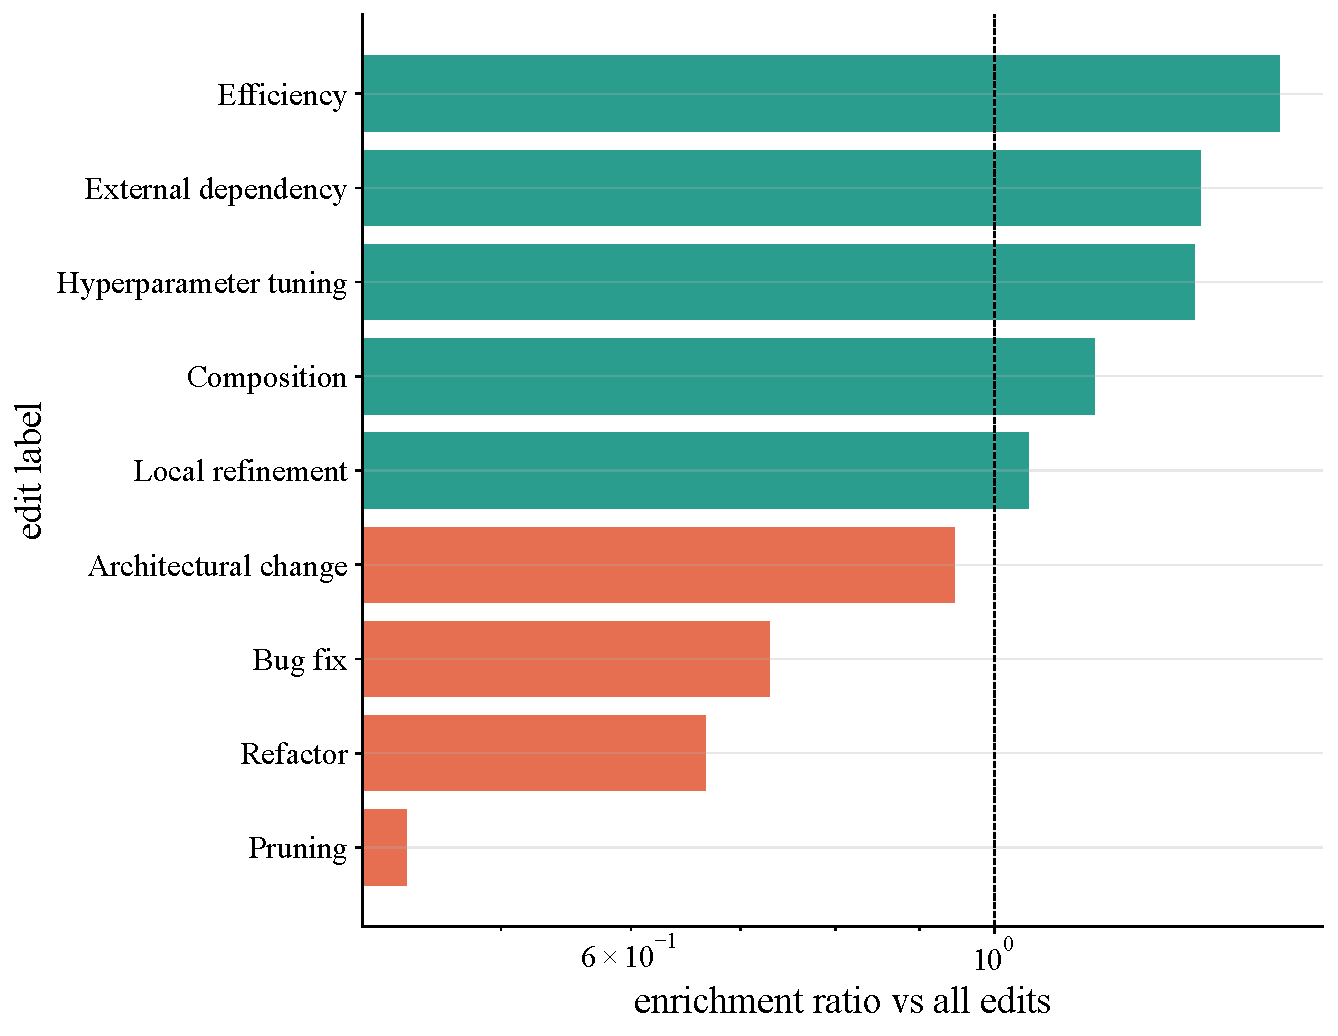
\includegraphics[width=0.6\linewidth]{paper_package_edits/main_figures/edit_enrichment_best_so_far.pdf}
\caption{\textbf{Best-so-far enrichment of edit labels (aggregate).} Enrichment of each taxonomy label among best-so-far updates relative to the all-edits base rate. The categories most overrepresented on successful intermediate steps (\emph{Efficiency}, \emph{External dependency}, \emph{Hyperparameter tuning}, \emph{Composition}) are not identical to the most frequent labels in Figure~\ref{fig:edit-taxonomy-results}~(a).}
\label{fig:edit-bsf-enrichment-aggregate}
\end{figure}

\begin{figure}[h]
\centering
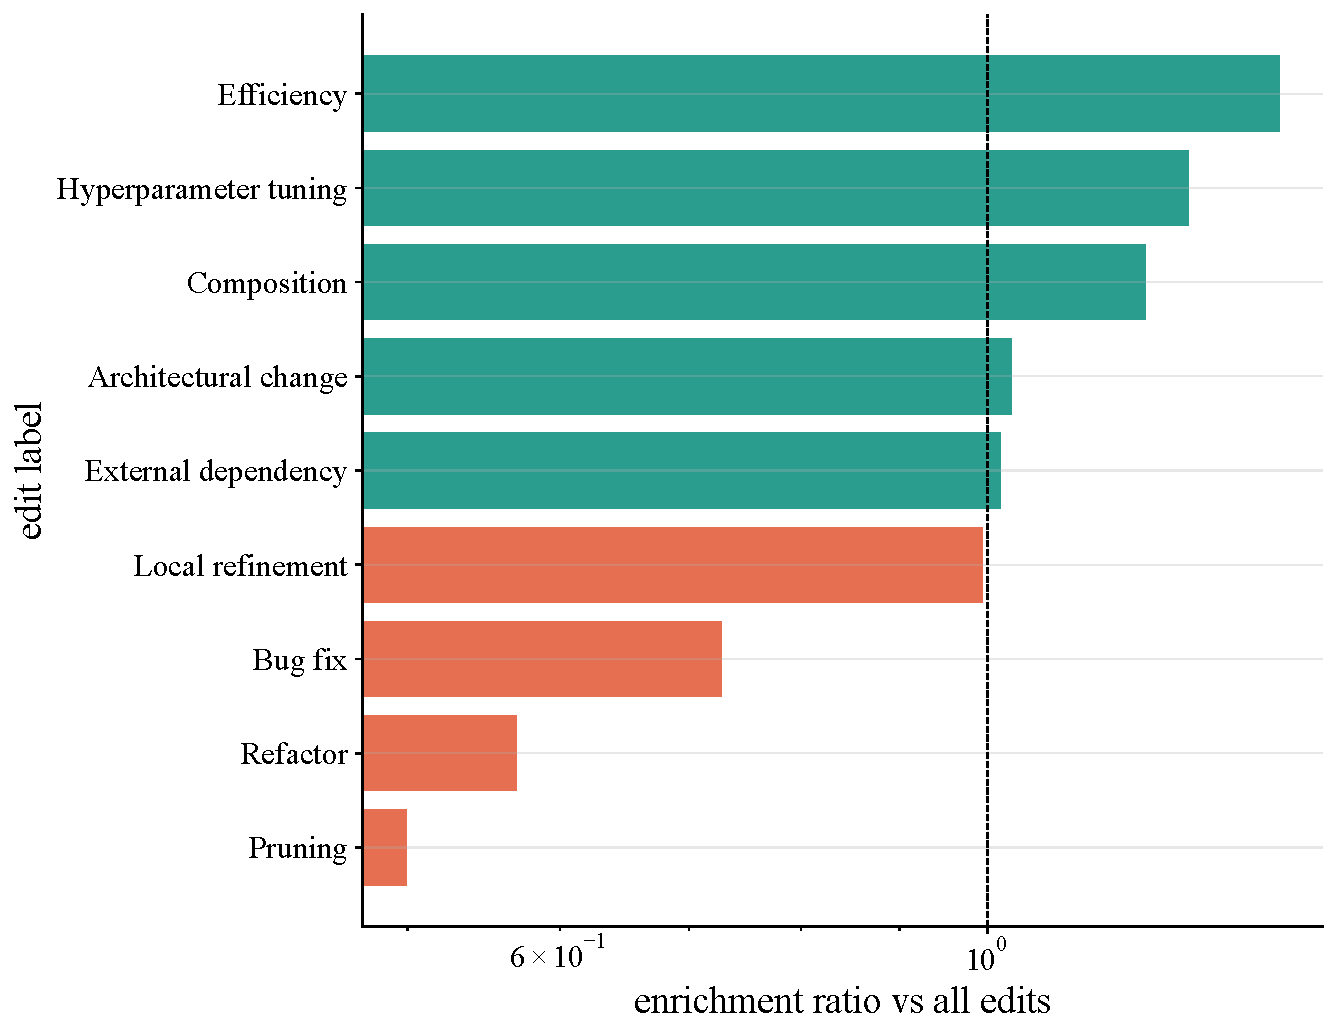
\includegraphics[width=0.6\linewidth]{paper_package_edits/main_figures/edit_enrichment_final_best_lineage.pdf}
\caption{\textbf{Final-best-lineage enrichment (aggregate, robustness check).} Enrichment of each label along the lineage from each run's final best program back to the seed. \emph{Efficiency}, \emph{Hyperparameter tuning}, and \emph{Composition} remain overrepresented relative to the all-edits base rate, supporting the best-so-far view in Figure~\ref{fig:edit-bsf-enrichment-aggregate}.}
\label{fig:edit-final-best-enrichment-aggregate}
\end{figure}

\subsection{Edit-taxonomy breakdowns by domain and backend}
\label{appendix:edit-taxonomy-breakdowns}

The aggregate edit-taxonomy results reported in \S\ref{sec:static-analysis} (Figure~\ref{fig:edit-taxonomy-results}) combine ALE and math runs across all four backends. This section reports the same analyses split by domain and, for the helpfulness view, by backend, so that readers can verify that the headline patterns survive these slices. The underlying labeled corpus covers all programs in EvoTrace.

\begin{figure}[h]
\centering
\begin{minipage}[b]{0.49\linewidth}
  \centering
  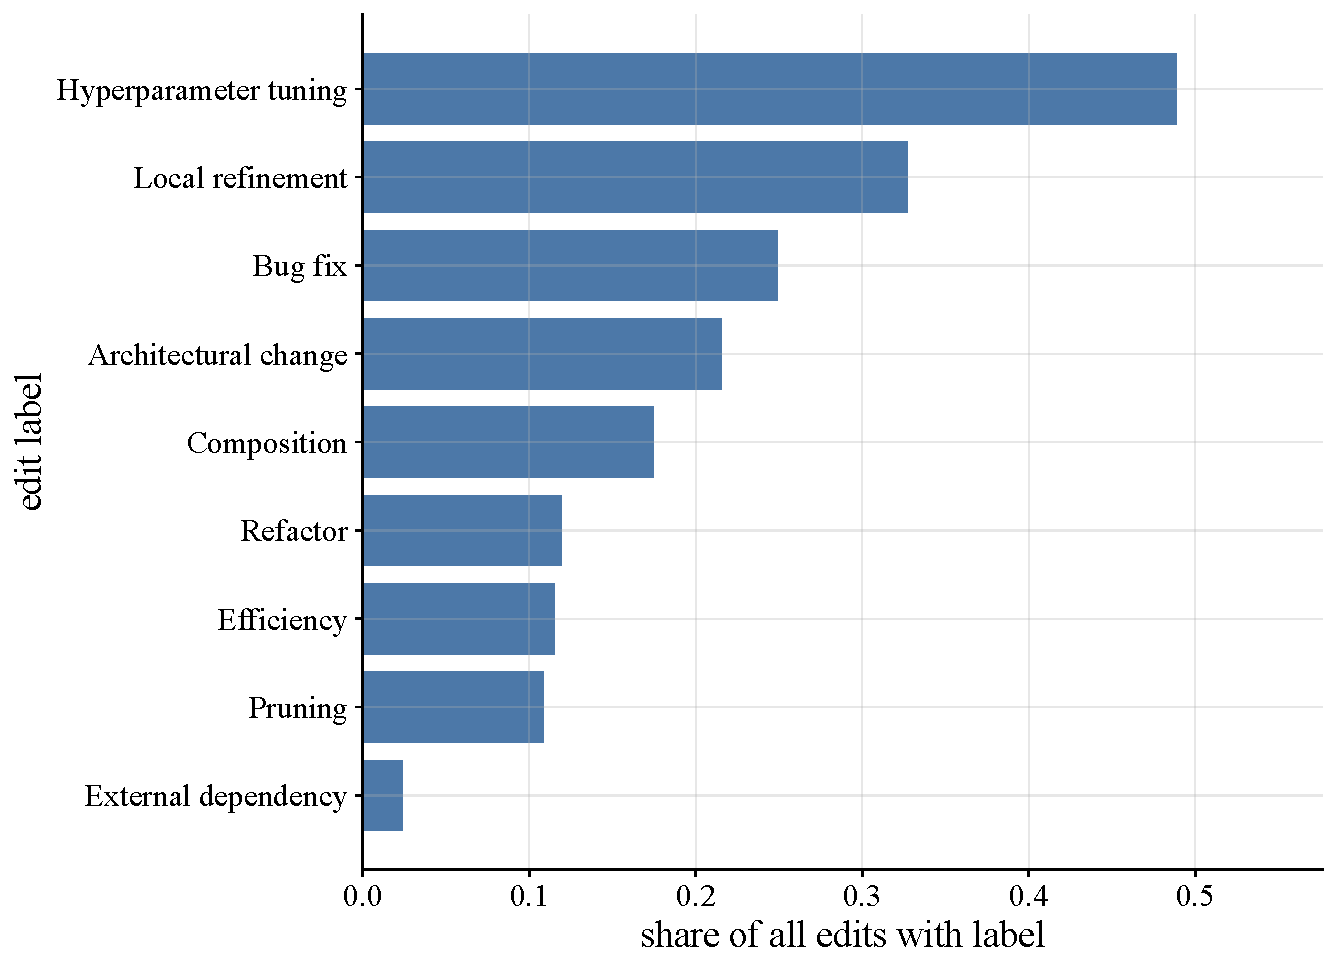
\includegraphics[width=\linewidth]{paper_package_edits/appendix_figures/edit_label_prevalence_ale.pdf}\\
  {\small (a) ALE}
\end{minipage}\hfill
\begin{minipage}[b]{0.49\linewidth}
  \centering
  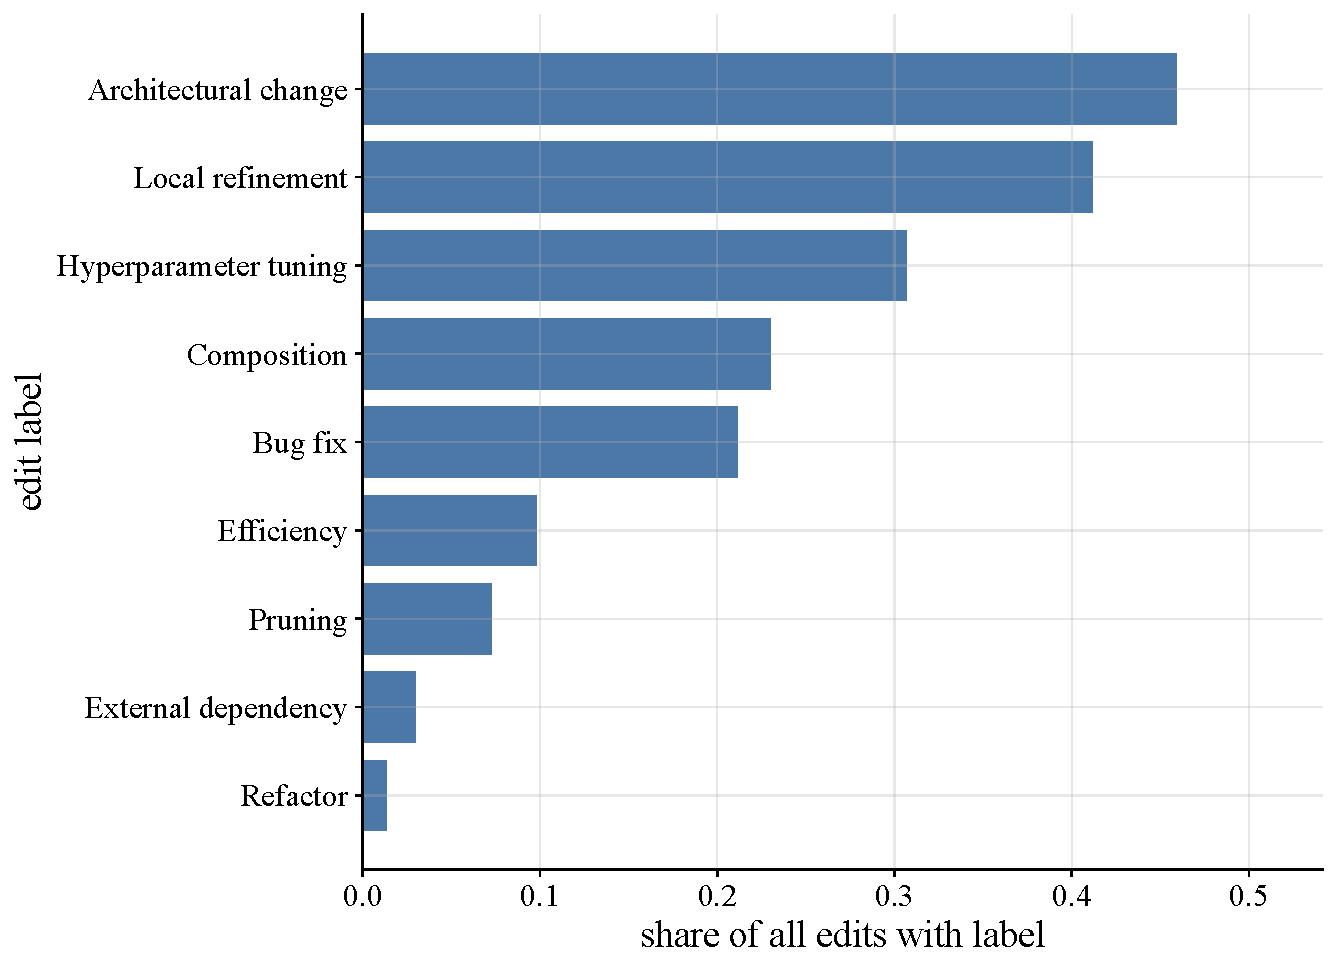
\includegraphics[width=\linewidth]{paper_package_edits/appendix_figures/edit_label_prevalence_math.pdf}\\
  {\small (b) Math}
\end{minipage}
\caption{\textbf{Edit-label prevalence by domain.} Frequency of each taxonomy label among labeled edits, split by domain. \emph{Hyperparameter tuning} dominates in both domains, but \emph{Composition} is more prominent on math while structural categories shift their relative weights between domains.}
\label{fig:edit-prevalence-by-domain}
\end{figure}

\begin{figure}[h]
\centering
\begin{minipage}[b]{0.49\linewidth}
  \centering
  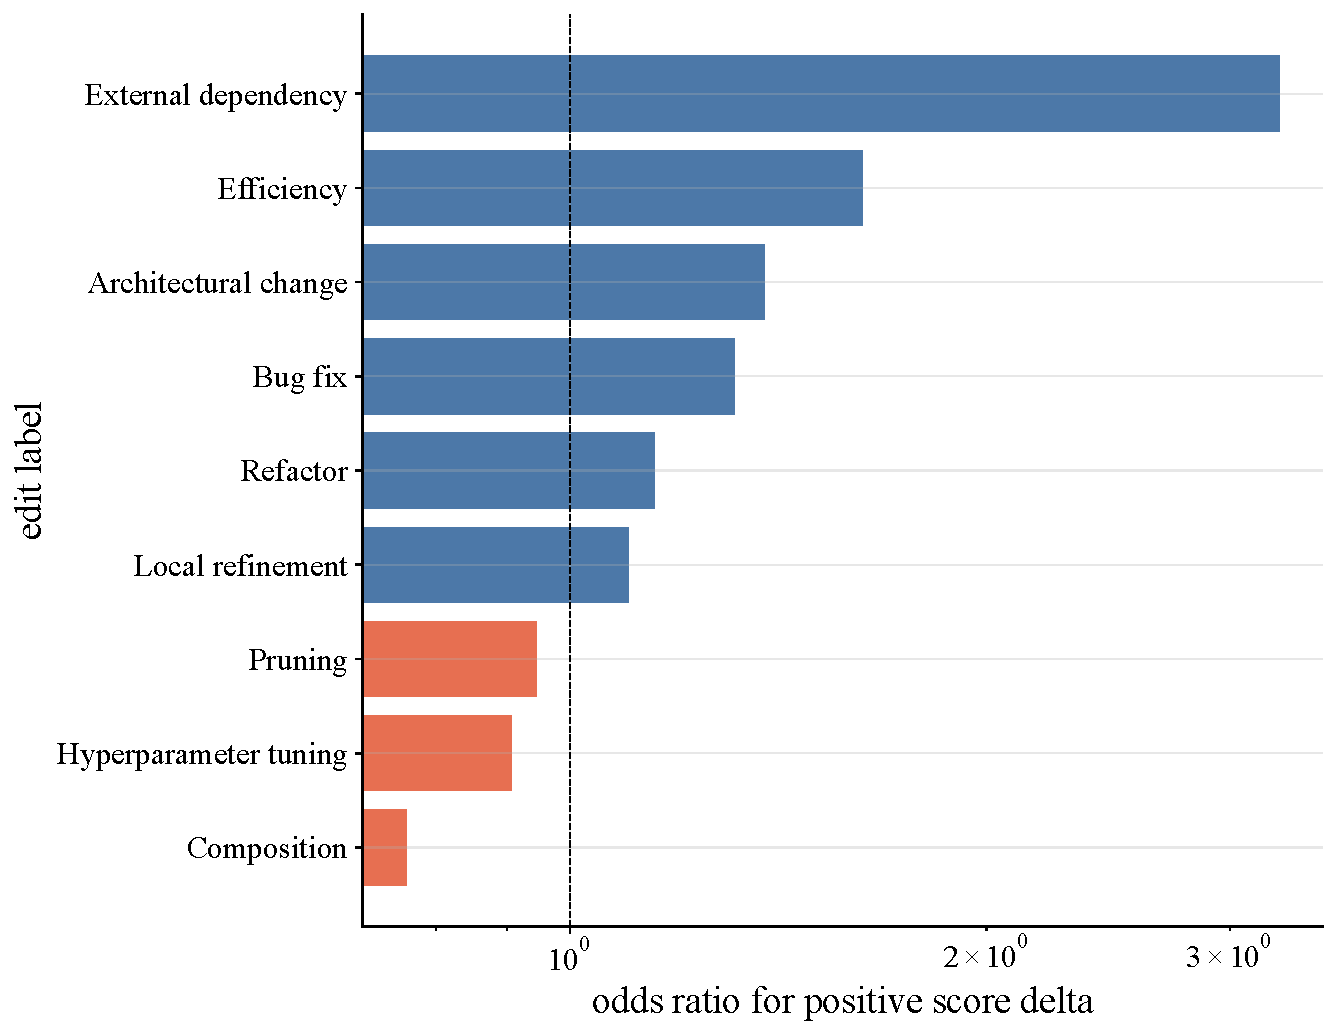
\includegraphics[width=\linewidth]{paper_package_edits/appendix_figures/edit_helpfulness_odds_ratio_ale.pdf}\\
  {\small (a) ALE}
\end{minipage}\hfill
\begin{minipage}[b]{0.49\linewidth}
  \centering
  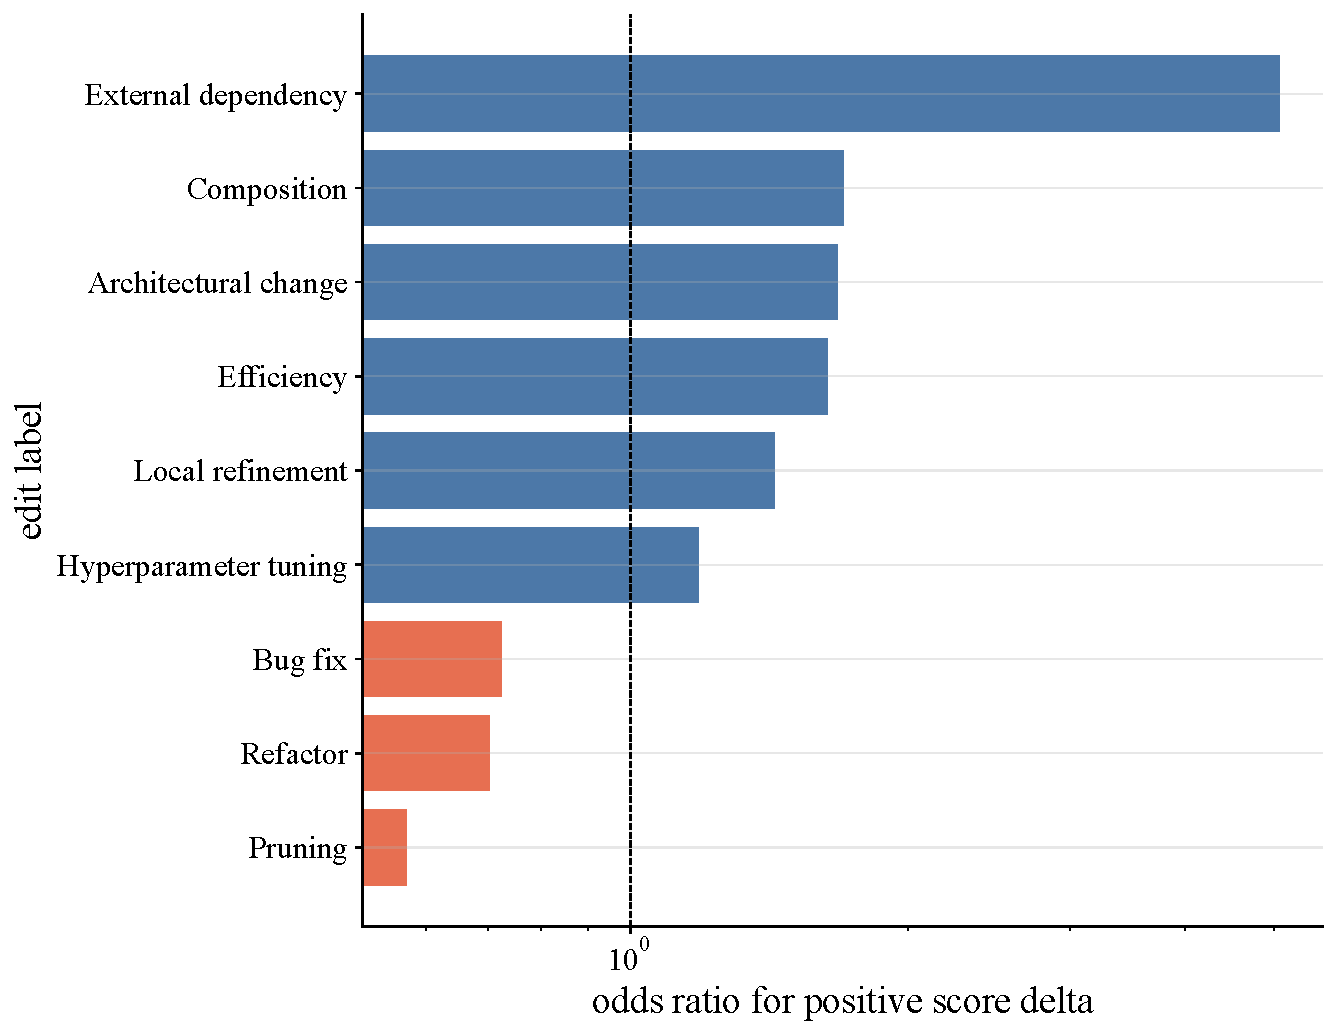
\includegraphics[width=\linewidth]{paper_package_edits/appendix_figures/edit_helpfulness_odds_ratio_math.pdf}\\
  {\small (b) Math}
\end{minipage}
\caption{\textbf{Per-edit helpfulness (odds ratio for positive normalized score change) by domain.} On ALE, \emph{External dependency}, \emph{Efficiency}, and \emph{Architectural change} are the strongest positive categories. On math, \emph{External dependency} is even stronger and \emph{Composition} plays a larger role than on ALE.}
\label{fig:edit-helpfulness-by-domain}
\end{figure}

\begin{figure}[h]
\centering
\begin{minipage}[b]{0.49\linewidth}
  \centering
  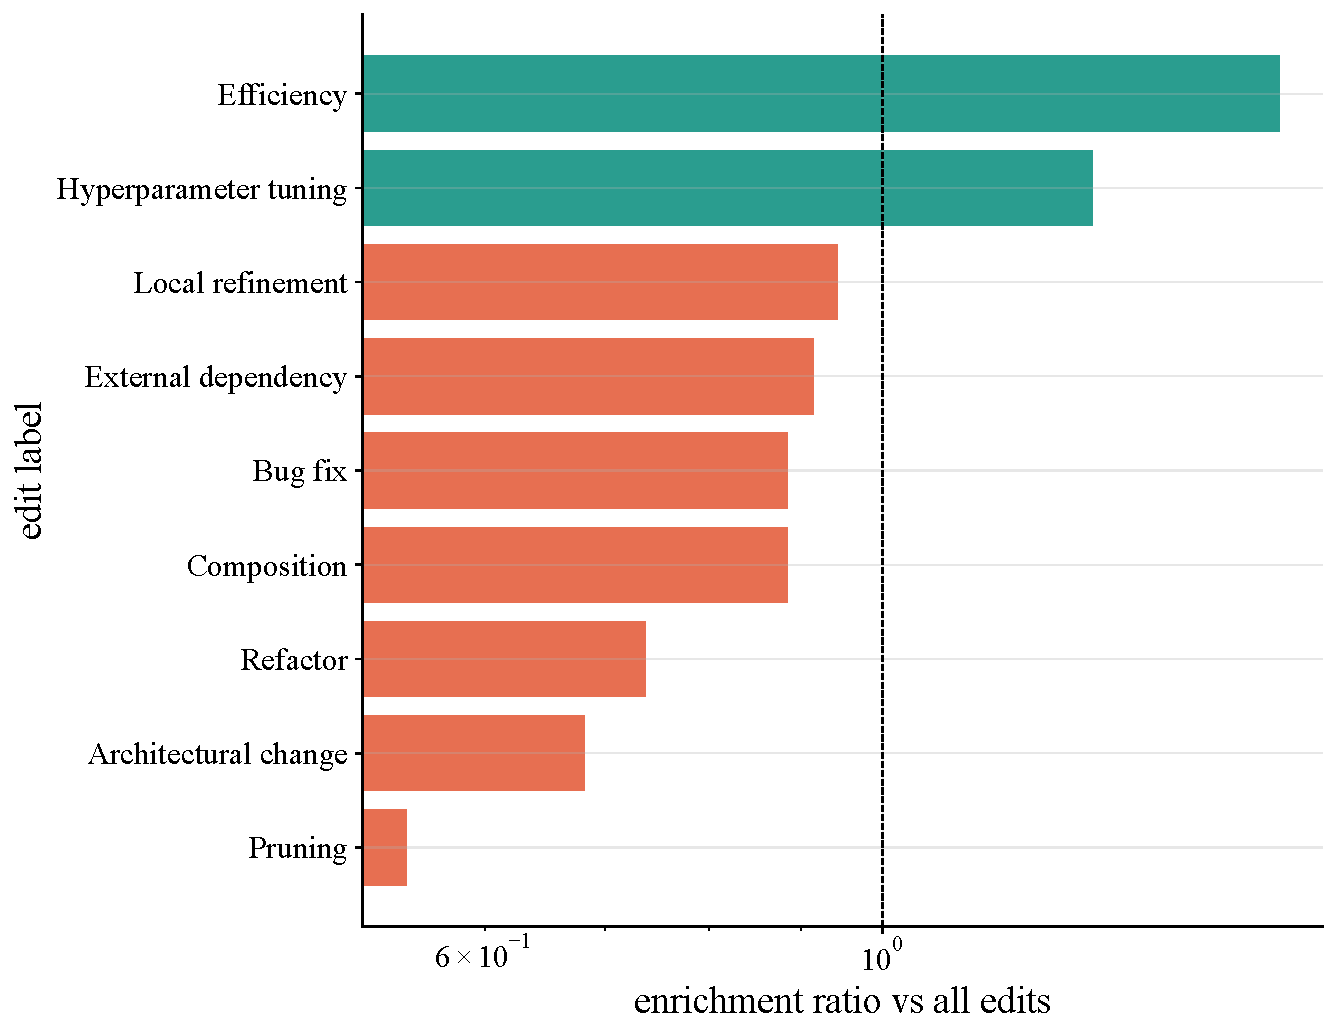
\includegraphics[width=\linewidth]{paper_package_edits/appendix_figures/edit_enrichment_best_so_far_ale.pdf}\\
  {\small (a) ALE}
\end{minipage}\hfill
\begin{minipage}[b]{0.49\linewidth}
  \centering
  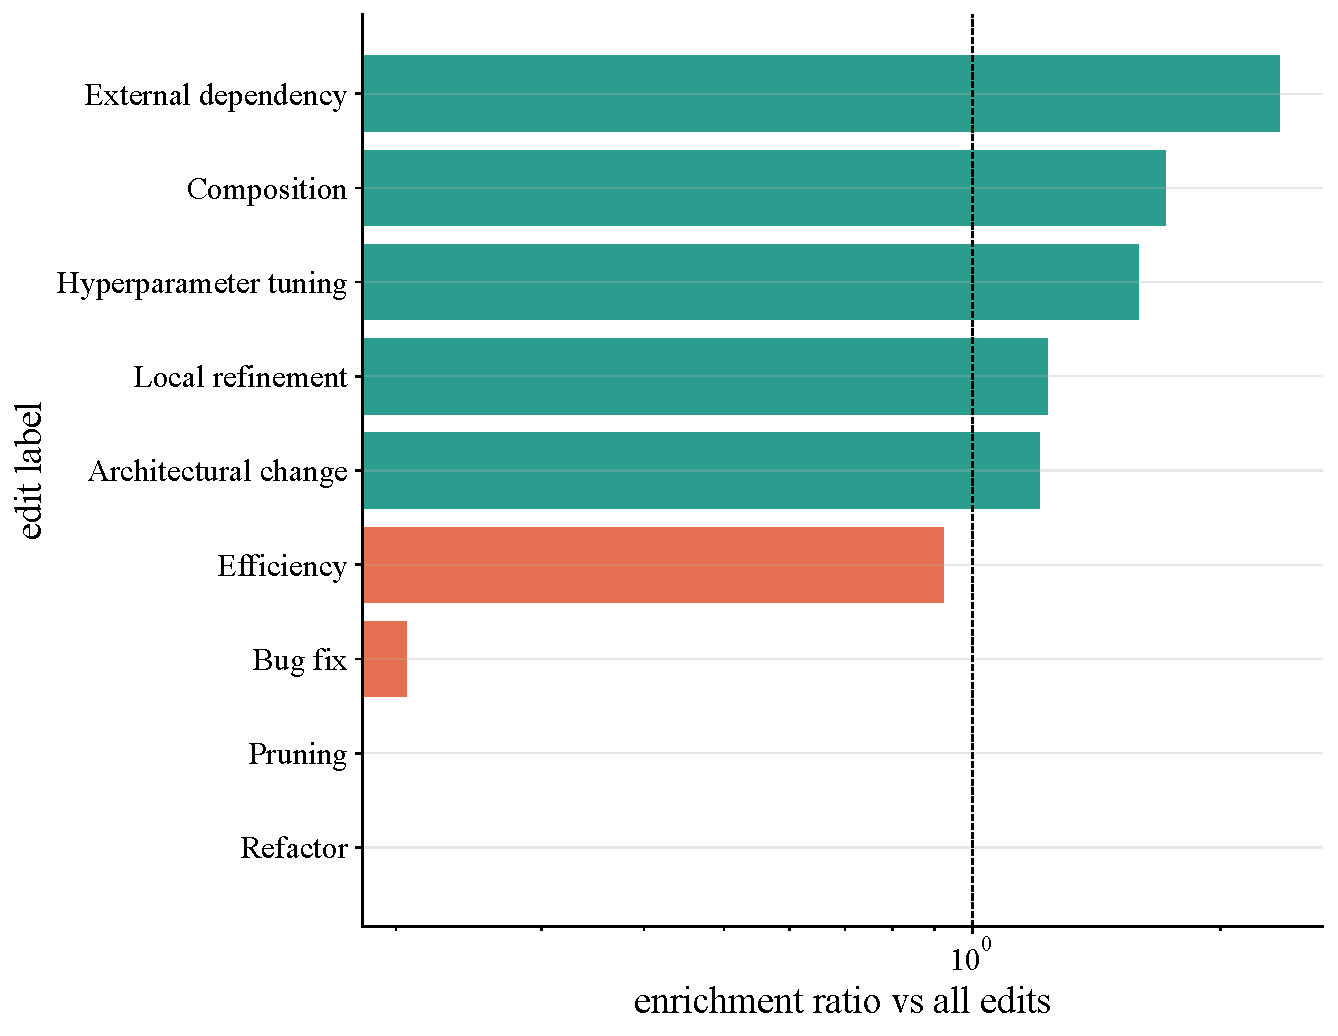
\includegraphics[width=\linewidth]{paper_package_edits/appendix_figures/edit_enrichment_best_so_far_math.pdf}\\
  {\small (b) Math}
\end{minipage}
\caption{\textbf{Best-so-far enrichment of edit labels by domain.} Enrichment of each label among best-so-far updates relative to the all-edits base rate, split by domain. The qualitative signal, a small set of categories (notably \emph{Efficiency}, \emph{External dependency}, and \emph{Hyperparameter tuning}) overrepresented on successful intermediate steps, is consistent with the aggregate view in Figure~\ref{fig:edit-taxonomy-results}, with domain-specific shifts in magnitude.}
\label{fig:edit-bsf-enrichment-by-domain}
\end{figure}

\begin{figure}[h]
\centering
\begin{minipage}[b]{0.49\linewidth}
  \centering
  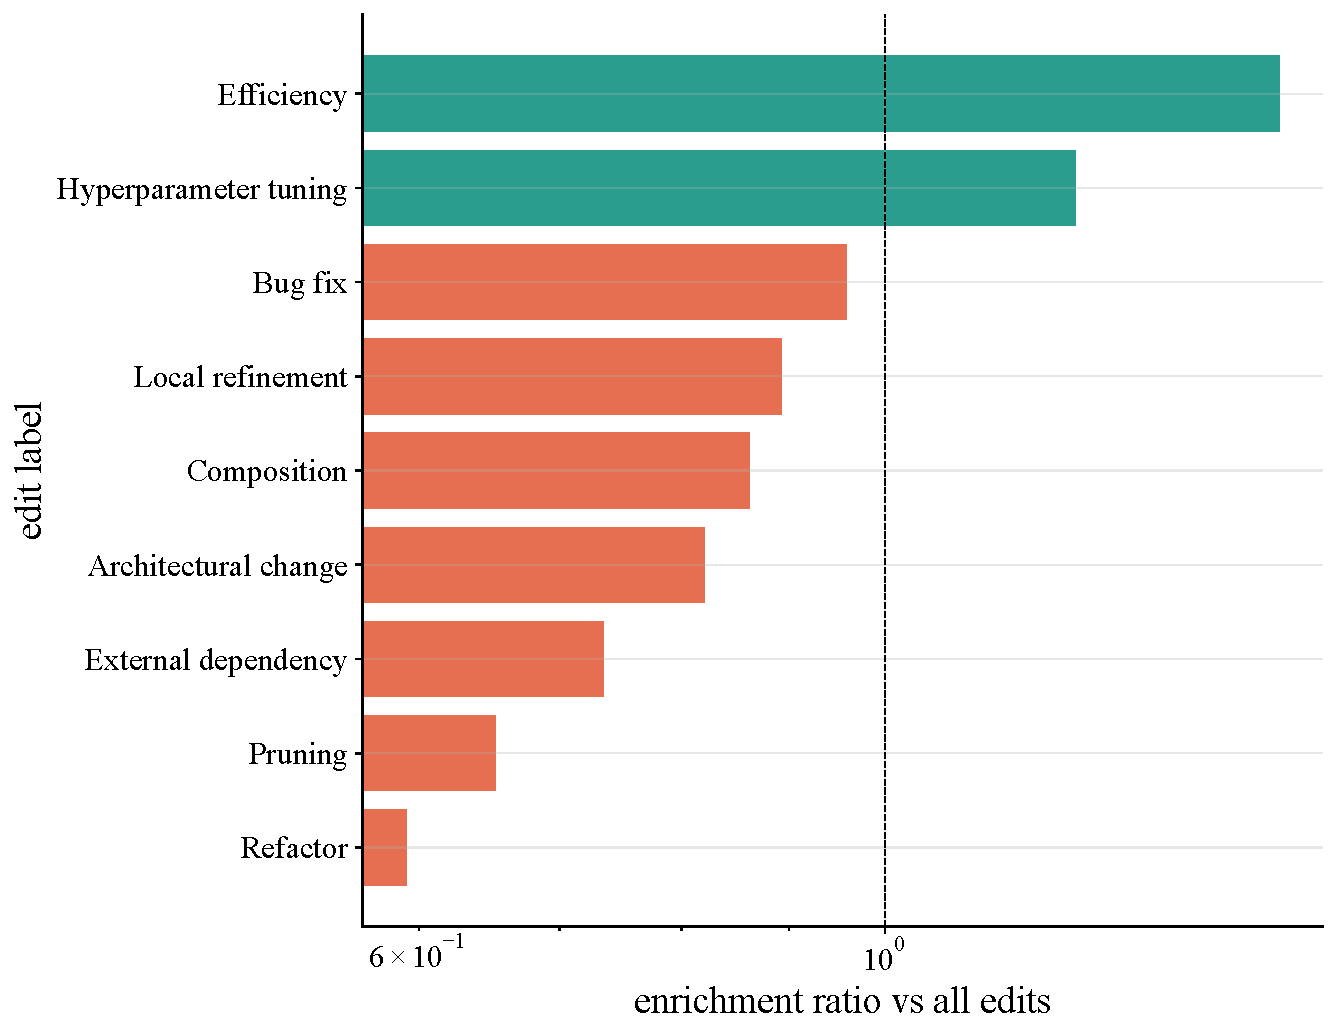
\includegraphics[width=\linewidth]{paper_package_edits/appendix_figures/edit_enrichment_final_best_lineage_ale.pdf}\\
  {\small (a) ALE}
\end{minipage}\hfill
\begin{minipage}[b]{0.49\linewidth}
  \centering
  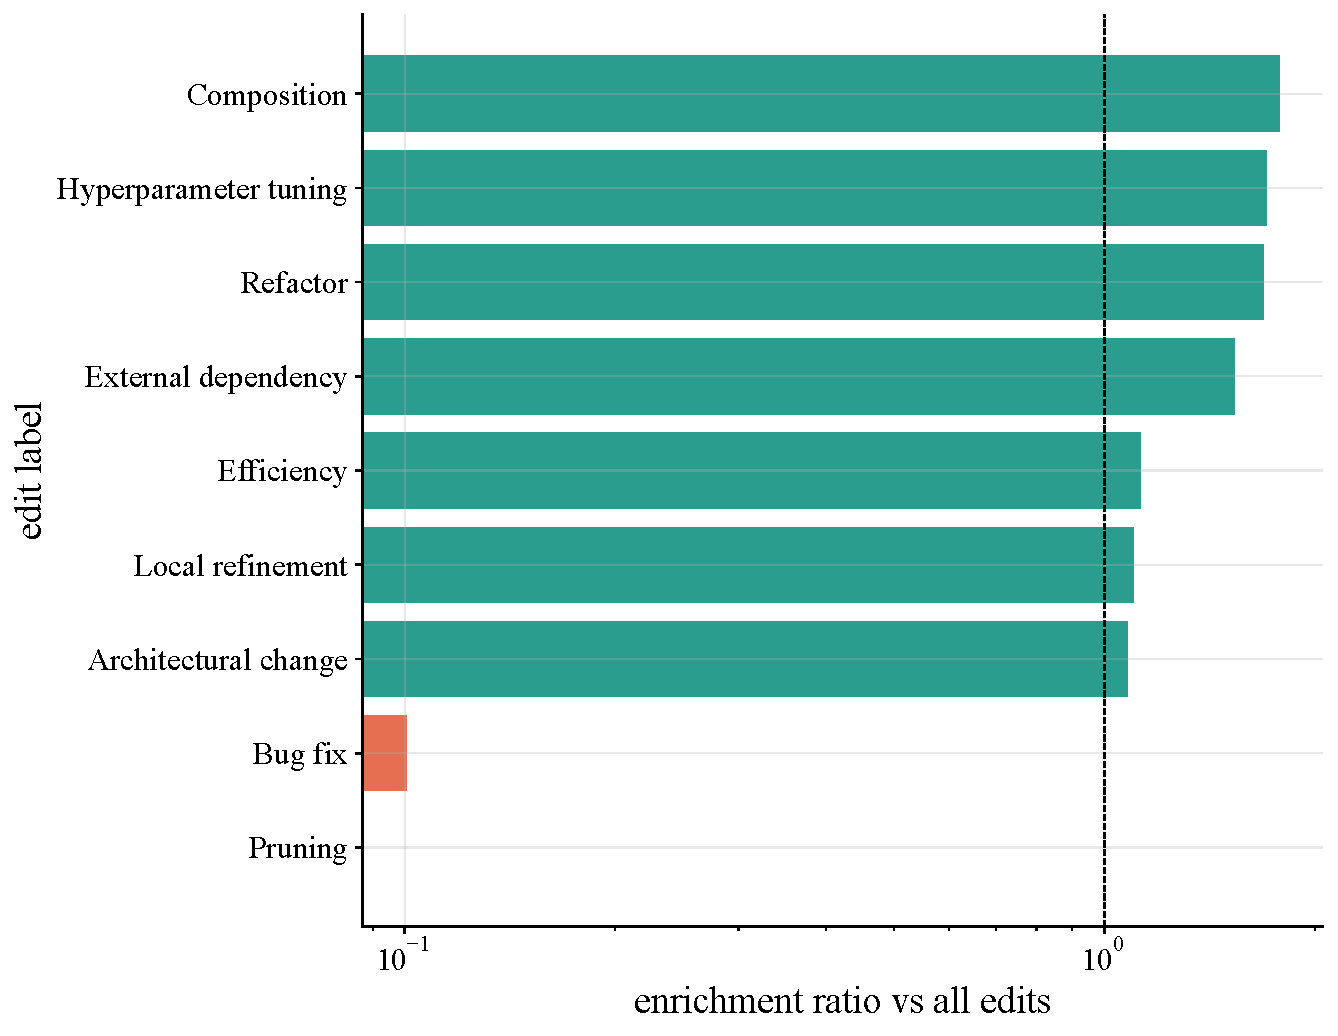
\includegraphics[width=\linewidth]{paper_package_edits/appendix_figures/edit_enrichment_final_best_lineage_math.pdf}\\
  {\small (b) Math}
\end{minipage}
\caption{\textbf{Final-best-lineage enrichment by domain.} Robustness check for Figure~\ref{fig:edit-bsf-enrichment-by-domain}, restricted to edits that lie on the lineage of each run's final best program. The enriched categories overlap heavily with the best-so-far view in both domains, with \emph{Efficiency} and \emph{Hyperparameter tuning} retaining their overrepresentation.}
\label{fig:edit-final-best-enrichment-by-domain}
\end{figure}

\begin{figure}[h]
\centering
\begin{minipage}[b]{0.49\linewidth}
  \centering
  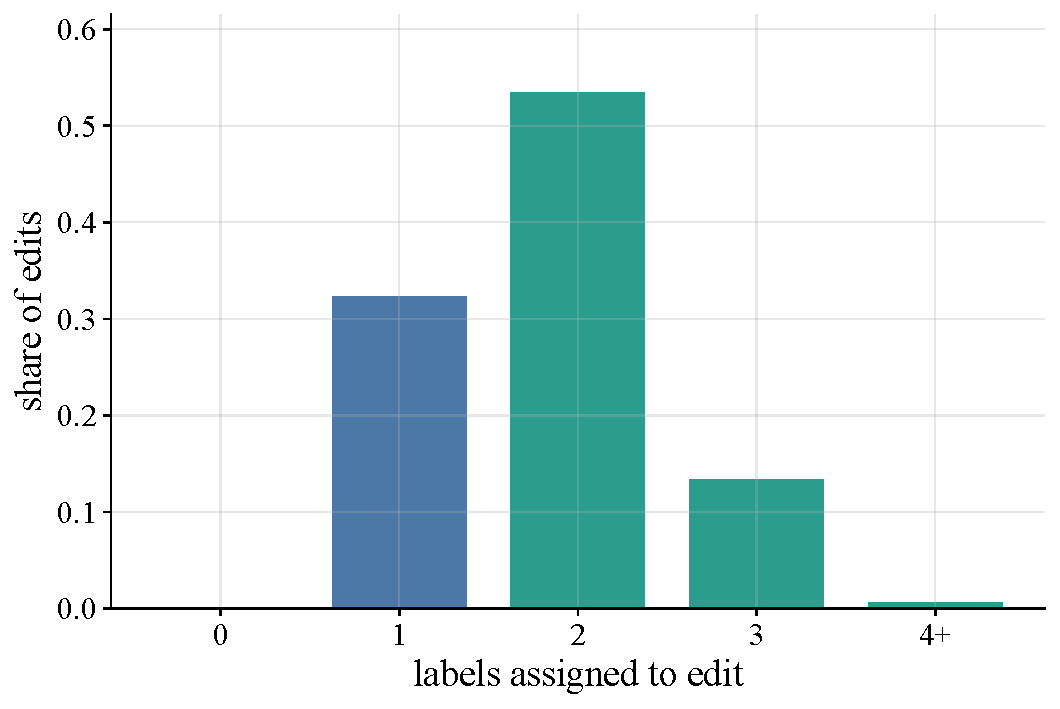
\includegraphics[width=\linewidth]{paper_package_edits/appendix_figures/edit_label_count_distribution_ale.pdf}\\
  {\small (a) ALE}
\end{minipage}\hfill
\begin{minipage}[b]{0.49\linewidth}
  \centering
  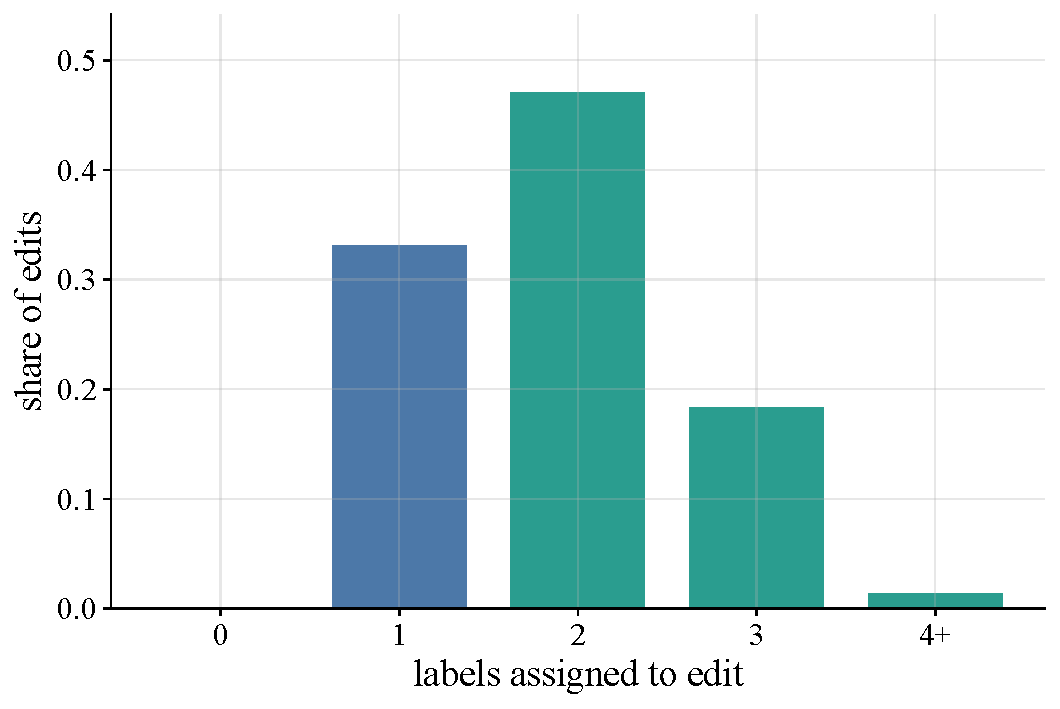
\includegraphics[width=\linewidth]{paper_package_edits/appendix_figures/edit_label_count_distribution_math.pdf}\\
  {\small (b) Math}
\end{minipage}
\caption{\textbf{Distribution of labels per edit, by domain.} Most edits in both domains are multi-label: $52.4\%$ of edits aggregate-wide carry exactly two labels and only $32.4\%$ are single-label. The categories of Figure~\ref{fig:edit-taxonomy-results} should therefore be read as overlapping rather than mutually exclusive modes.}
\label{fig:edit-label-count-by-domain}
\end{figure}

\begin{figure}[h]
\centering
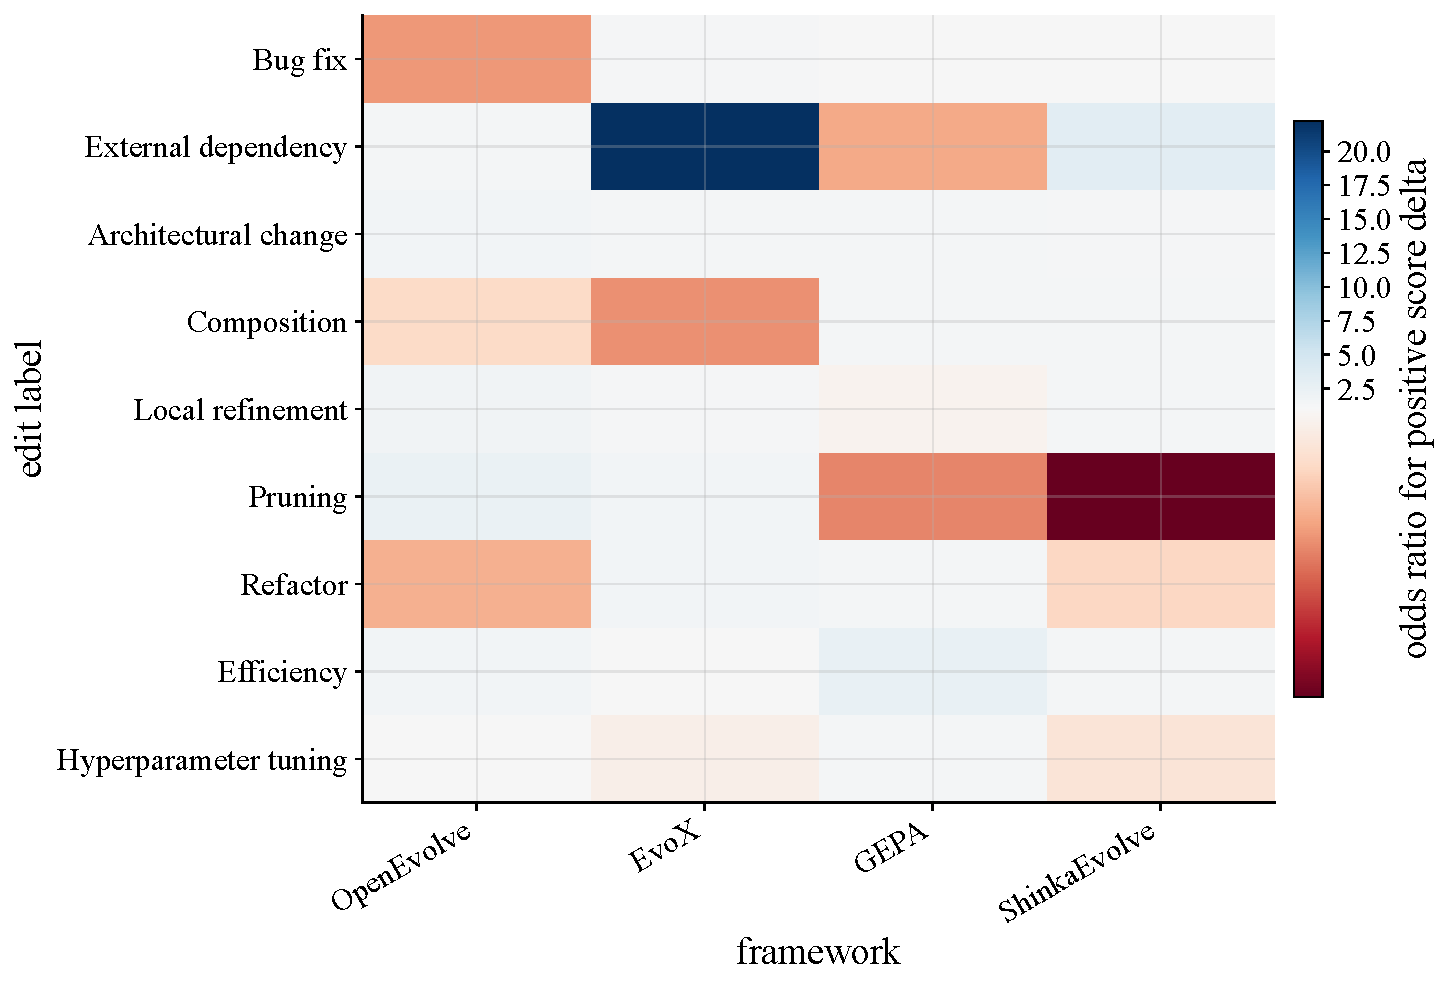
\includegraphics[width=0.85\linewidth]{paper_package_edits/appendix_figures/edit_helpfulness_odds_ratio_by_backend.pdf}
\caption{\textbf{Per-edit helpfulness by backend.} Odds ratio for positive normalized score change broken down by the four evolutionary backends. Some categories (notably \emph{External dependency}) are consistently positive across backends, while others vary in magnitude. \texttt{openevolve\_native} contributes only $2$ runs to this corpus, so its column should be interpreted with a wider implicit confidence band; we include it for completeness.}
\label{fig:edit-helpfulness-by-backend}
\end{figure}

\subsection{LLM-as-judge validation}
\label{appendix:judge-validation}

\paragraph{Taxonomy origin.}
The 9-category edit taxonomy used in \S\ref{sec:static-analysis} was derived inductively from EvoTrace runs rather than imposed top-down. The first author sampled several classified runs and proposed an initial set of edit categories; these were discussed and refined with co-authors over multiple iterations on further sampled traces, with categories merged or split until the label set stabilised on the nine used to prompt the LLM judge: \emph{hyperparameter\_tuning}, \emph{local\_refinement}, \emph{architectural\_change}, \emph{composition}, \emph{efficiency}, \emph{bug\_fix}, \emph{pruning}, \emph{refactor}, and \emph{external\_dependency}. Table~\ref{tab:edit-type-definitions} gives a one-line working definition for each label; curated example diffs are provided in Appendix~\ref{appendix:edit-examples}.

\begin{table}[h]
\centering
\caption{Working definitions of the nine edit categories. One curated example diff per category is given in Appendix~\ref{appendix:edit-examples}.}
\label{tab:edit-type-definitions}
\small
\renewcommand{\arraystretch}{1.25}
\begin{tabular}{@{}lp{0.72\linewidth}@{}}
\toprule
\textbf{Label} & \textbf{Definition} \\
\midrule
Hyperparameter tuning & Change to one or more numeric literals or configuration values; control flow and surrounding algorithm unchanged. \\
Local refinement      & Targeted edit within an existing routine; the routine's role and structure are preserved. \\
Architectural change  & A core algorithmic block is replaced by a substantively different approach. \\
Composition           & A new component (operator, phase, branch) is added alongside an existing one; existing logic is retained. \\
Efficiency            & Same input--output behaviour reimplemented at lower asymptotic or constant cost (e.g.\ batching, vectorization, partial sorts, caching). \\
Bug fix               & Correction of a latent defect such as a missing guard, wrong sign, off-by-one, or mishandled sentinel. \\
Pruning               & A code path, phase, or feature is removed; the remaining program is kept intact. \\
Refactor              & Behaviour-preserving restructuring: renaming, reordering, extracting helpers, or moving declarations. \\
External dependency   & Introduction or removal of an import or external library. \\
\bottomrule
\end{tabular}
\end{table}

\paragraph{Inter-rater reliability against the LLM judge.}
To validate the LLM-as-judge classifier we conducted a blind multi-label inter-rater reliability study on a stratified sample of $200$ parent$\to$child edits drawn from three classified runs. The first author labelled each edit without seeing the model's output; agreement was then computed against the \texttt{deepseek-chat} judge.

Across the nine categories we observed substantial overall agreement: macro Cohen's $\kappa = 0.77$, mean Jaccard $= 0.86$, micro-$F_1 = 0.90$, and exact-match accuracy $= 74.5\%$.
\subsection{Curated examples per edit type}
\label{appendix:edit-examples}

To make the taxonomy labels of \S\ref{sec:static-analysis} concrete, we illustrate each of the nine categories with one curated example diff drawn from the labeled corpus. Examples are selected for visual clarity rather than for the highest score delta; some carry more than one label (e.g., \emph{Pruning}, \emph{Composition}, \emph{Bug fix}, \emph{Efficiency}, and \emph{External dependency} are each accompanied by other labels in the cleanest paper-ready example), which is itself part of the empirical story analyzed in Appendix~\ref{appendix:edit-taxonomy-breakdowns}: most edits in the corpus are multi-label. Each example below lists run identity, iteration, label set, and score delta; full unified diffs and metadata are bundled with the dataset release.

\paragraph{Hyperparameter tuning.}
\textit{Single cooling-rate change.} \texttt{openevolve\_native} / \texttt{heilbronn\_triangle}, iter $40$, labels $\{\text{hyperparameter\_tuning}\}$, $\Delta s = +0.0153$. The cleanest possible single-knob example: one numeric literal changes; the surrounding algorithm is unchanged.
{\scriptsize
\begin{verbatim}
@@ -74,7 +74,7 @@
     num_restarts = 25            # more restarts to escape local minima
     steps_per_run = 200000       # longer runs for better convergence
     T0 = 0.12                    # higher initial temperature
-    cooling_rate = 0.99992       # slightly slower cooling
+    cooling_rate = 0.99993       # slightly slower cooling (compensate more steps)
     best_min = 0.0
     best_points = None
\end{verbatim}
}

\paragraph{Pruning.}
\textit{Delete final global-shake phase.} \texttt{openevolve\_native} / \texttt{heilbronn\_triangle}, iter $38$, labels $\{\text{hyperparameter\_tuning},\,\text{pruning}\}$, $\Delta s = +0.0670$. A whole final optimization phase is removed (not commented out or renamed); the diff also retunes several literals, so this is a pruning-plus-tuning compound example.
{\scriptsize
\begin{verbatim}
@@ -71,10 +71,10 @@
         return np.min(area)

     # Simulated Annealing parameters
-    num_restarts = 35            # increased restarts to escape local minima
-    steps_per_run = 250000       # longer runs for better convergence
-    T0 = 0.15                    # higher initial temperature for more exploration
-    cooling_rate = 0.99992       # slightly slower cooling
+    num_restarts = 25            # balanced restarts and run length
+    steps_per_run = 280000       # more steps for deeper exploration
+    T0 = 0.12                    # initial temperature
+    cooling_rate = 0.99993       # slightly slower cooling (compensate more steps)
     best_min = 0.0
     best_points = None

@@ -169,24 +169,6 @@
             best_min = current_min_ref
             best_points = points_ref.copy()

-    # Final global shake of best configuration to escape narrow local minima
-    if best_points is not None:
... [truncated, see full diff file] ...
\end{verbatim}
}

\paragraph{Architectural change.}
\textit{Brute-force candidate search replaced by closed-form selection.} \texttt{evox} / \texttt{ale\_bench\_ahc016}, iter $28$, labels $\{\text{architectural\_change},\,\text{local\_refinement}\}$, $\Delta s = +1.37 \times 10^{7}$. The program stops scanning many candidate graph sizes and switches to a derived closed-form rule.
{\scriptsize
\begin{verbatim}
@@ -203,40 +203,49 @@
     double epsilon_noise_rate;
     std::cin >> M_graphs >> epsilon_noise_rate;

-    double best_score = -1e100;
-    int best_N = 4;
-    Strategy best_strat = Strategy::GED;
-
-    // Evaluate GED strategies (N=4,5,6)
-    for (int Ncand : {4,5,6}) {
-        if (Ncand == 6 && M_graphs > 156) continue;
-        if (Ncand == 5 && M_graphs > 34) continue;
-        if (Ncand == 4 && M_graphs > 11) continue;
-        double score = estimate_ged_score(Ncand, M_graphs, epsilon_noise_rate);
-        if (score > best_score) { ... }
-    }
-    // Evaluate edge-count strategies (N=4..100)
-    for (int Ncand = 4; Ncand <= 100; ++Ncand) {
-        double score = estimate_edge_score(Ncand, M_graphs, epsilon_noise_rate);
-        if (score > best_score) { ... }
-    }
+    int N_for_GED_strat;
+    if (M_graphs <= 11) N_for_GED_strat = 4;
... [truncated, see full diff file] ...
\end{verbatim}
}

\paragraph{Local refinement.}
\textit{Add boundary bonus inside the existing scoring heuristic.} \texttt{evox} / \texttt{ale\_bench\_ahc015}, iter $94$, labels $\{\text{local\_refinement}\}$, $\Delta s = +4{,}295$. Small targeted change to a heuristic formula; surrounding algorithm intact.
{\scriptsize
\begin{verbatim}
@@ -283,6 +283,10 @@
                 if ((candy.c == 0 && min_target_c == 0) ||
                     (candy.c == GRID_SIZE - 1 && max_target_c == GRID_SIZE - 1)) {
                      bonus_val += PER_CANDY_BONUS_FACTOR;
+                }
+                // Additional bonus for being at the boundary of the target column range
+                if (candy.c == min_target_c || candy.c == max_target_c) {
+                    bonus_val += 0.5;
                 }
             }
         }
\end{verbatim}
}

\paragraph{Composition.}
\textit{Add swap mutation operator on top of existing plan search.} \texttt{evox} / \texttt{ale\_bench\_ahc026}, iter $57$, labels $\{\text{hyperparameter\_tuning},\,\text{composition}\}$, $\Delta s = +9{,}252$. Main search intact; an additional mutation operator is layered on, alongside several constant retunings.
{\scriptsize
\begin{verbatim}
@@ -18,11 +18,11 @@
 // Constants for heuristic evaluation
-const double HEURISTIC_EMPTY_STACK_BONUS_SCORE = 1500.0;
+const double HEURISTIC_EMPTY_STACK_BONUS_SCORE = 1000.0;
 const double STACK_HEIGHT_PENALTY_FACTOR = 0.1;
 const int    HEURISTIC_LOOKAHEAD_WINDOW = 5;
-const double HEURISTIC_COVER_CRITICAL_PENALTY_PER_BOX_ABOVE = 4.0;
-const double HEURISTIC_MIN_LABEL_IN_DEST_FACTOR = 0.03;
+const double HEURISTIC_COVER_CRITICAL_PENALTY_PER_BOX_ABOVE = 5.0;
+const double HEURISTIC_MIN_LABEL_IN_DEST_FACTOR = 0.05;

@@ -473,7 +467,7 @@
         double op_choice_rand = RGen.a_double(0.0, 1.0);
-        if (op_choice_rand < 0.35 && N_CONST > 0) {
+        if (op_choice_rand < 0.25 && N_CONST > 0) {
... [truncated, see full diff file] ...
\end{verbatim}
}

\paragraph{Bug fix.}
\textit{Check strategy success and INF\_COST sentinel.} \texttt{evox} / \texttt{ale\_bench\_ahc046}, iter $99$, labels $\{\text{bug\_fix},\,\text{hyperparameter\_tuning}\}$, $\Delta s = +56.2$. Parent silently ignored a helper's return value and invalid-cost sentinel; child explicitly guards against both failure modes.
{\scriptsize
\begin{verbatim}
@@ -378,7 +378,7 @@
-const int GREEDY_REOPTIMIZE_SUBSET_SIZE = 40;  // Balanced between exploration and speed
+const int GREEDY_REOPTIMIZE_SUBSET_SIZE = 170; // Full scan for best strategy per segment

@@ -798,12 +798,16 @@
             current_sa_choices[k] = current_best_strategy_code_for_k;

             SegmentExecResult final_segment_res_for_k_build;
-            apply_combined_strategy(current_best_strategy_code_for_k,
+            bool success_seg = apply_combined_strategy(
+                                    current_best_strategy_code_for_k,
                                     player_pos_sim_build,
                                     target_P_k,
                                     greedy_grid_sim_build,
                                     final_segment_res_for_k_build,
                                     true);
+            if (!success_seg || final_segment_res_for_k_build.turns == INF_COST) {
+                possible_greedy = false;
+                break;
+            }
\end{verbatim}
}

\paragraph{Efficiency.}
\textit{\texttt{std::sort} replaced by \texttt{std::nth\_element}.} \texttt{evox} / \texttt{ale\_bench\_ahc027}, iter $46$, labels $\{\text{efficiency},\,\text{hyperparameter\_tuning}\}$, $\Delta s \approx 9.2 \times 10^{18}$. Top-$k$ selection semantics are preserved; full sort is replaced by a partial-ordering primitive.
{\scriptsize
\begin{verbatim}
@@ -266,8 +266,6 @@
              TMP_CELL_DIRT_INFOS_LIST_GLOBAL_BUFFER.push_back(...);
         }
     }
-    std::sort(TMP_CELL_DIRT_INFOS_LIST_GLOBAL_BUFFER.begin(),
-              TMP_CELL_DIRT_INFOS_LIST_GLOBAL_BUFFER.end());

@@ -275,6 +273,13 @@
     // Stochastic: pick uniformly from the top 20% of cells
     int num_candidates = std::max(1,
         (int)TMP_CELL_DIRT_INFOS_LIST_GLOBAL_BUFFER.size() / 5);
+    // Use nth_element to partition: the first num_candidates elements are the largest
+    std::nth_element(TMP_CELL_DIRT_INFOS_LIST_GLOBAL_BUFFER.begin(),
+                     TMP_CELL_DIRT_INFOS_LIST_GLOBAL_BUFFER.begin() + num_candidates,
+                     TMP_CELL_DIRT_INFOS_LIST_GLOBAL_BUFFER.end(),
+                     [](const CellDirtInfo& a, const CellDirtInfo& b) {
+                         return a.weighted_dirt_contribution
+                              > b.weighted_dirt_contribution;
+                     });

@@ -600,7 +605,7 @@
-        const int POST_MAX_ATTEMPTS = 500;
+        const int POST_MAX_ATTEMPTS = 200;
\end{verbatim}
}

\paragraph{External dependency.}
\textit{Introduce JAX and Optax optimization pipeline.} \texttt{shinkaevolve} / \texttt{first\_autocorr\_ineq}, iter $94$, labels $\{\text{architectural\_change},\,\text{external\_dependency}\}$, $\Delta s = +0.991$. The strongest paper example of \emph{external\_dependency}: the imports of \texttt{jax} and \texttt{optax} are unambiguous and visually prominent. Note that the same diff also constitutes a large architectural change, illustrating that this label often appears in combination with others.
{\scriptsize
\begin{verbatim}
@@ -1,3 +1,127 @@
 # EVOLVE-BLOCK-START
-# Paste your original program here. Ensure the evolve block markers are present.
+import jax
+import jax.numpy as jnp
+import optax
+import numpy as np
+from dataclasses import dataclass
+
+@dataclass
+class Hyperparameters:
+    num_intervals: int = 600
+    learning_rate: float = 0.005
+    end_lr_factor: float = 1e-4
+    num_steps: int = 40000
+    warmup_steps: int = 2000
+
+class AutocorrelationOptimizer:
+    def __init__(self, hypers: Hyperparameters):
+        self.hypers = hypers
+        self.domain_width = 0.5
+        self.dx = self.domain_width / self.hypers.num_intervals
... [truncated, see full diff file] ...
\end{verbatim}
}

\paragraph{Refactor.}
\textit{Move \texttt{SimulationResult} definition before use.} \texttt{shinkaevolve} / \texttt{ale\_bench\_ahc026}, iter $68$, labels $\{\text{refactor}\}$, $\Delta s = +9{,}248$. The cleanest refactor diff in the corpus: a type definition is moved to a more appropriate place without changing the algorithm or introducing new logic.
{\scriptsize
\begin{verbatim}
@@ -137,7 +137,13 @@
     }
 };

-// Forward declaration for helper functions
+// Define SimulationResult before any function that uses it
+struct SimulationResult {
+    long long energy_cost;
+    std::vector<std::pair<int, int>> ops_history;
+};
+
+// Forward declaration for helper functions (SimulationResult is now defined)
 std::pair<State, long long> simulate_up_to_k(
     const std::vector<std::vector<int>>& init,
     const std::vector<int>& plan,

@@ -319,11 +325,6 @@
     return run_simulation_from_intermediate_state(
         std::move(st), plan, 0, N, M, record_all);
 }

-struct SimulationResult {
-    long long energy_cost;
-    std::vector<std::pair<int, int>> ops_history;
-};
-
 int main() {
\end{verbatim}
}

\subsection{Cycling: additional analyses}
\label{appendix:cycling-extras}

The body section \S\ref{sec:cycling} reports only the headline cycling result. This appendix covers (i) a finer three-way classifier on the unified diff, (ii) a model- and prompt-dependence breakdown of the tuning share, and (iii) a null result on post-breakthrough cycling that did not survive cross-run aggregation.

\paragraph{Three-way classifier.}
Each parent--child edit is classified deterministically using three categories on the unified diff between $\mathbf{p}_t$ and $p_t$. \emph{Literal recycling}: the added line is byte-identical to a line previously removed elsewhere in the lineage. \emph{Tuning recycling}: the added line's number-collapsed skeleton matches a previously-removed line, but the numeric values differ (coefficient churn). \emph{Trivial recycling}: comment-only or whitespace-only changes. The body cycling rate aggregates all three; per-category rates are emitted by the classifier.

\paragraph{Edit composition is model- and prompt-dependent.}
Restricting to code-changing lines, the median per-run share that the paired-skeleton classifier marks as \emph{tuning recycling} is $8\%$, but the range is wide ($2$--$44\%$). Holding the task fixed at \texttt{ahc015}, the tuning share varies sharply with the generator (Table~\ref{tab:tuning-share-ahc015}). The diff-vs-no-diff axis is the strongest single predictor: the same model (\texttt{deepseek-reasoner}) drops from $20\%$ to $2\%$ tuning share when its diff-based generation is turned off.

\begin{table}[h]
\centering
\caption{Tuning share of code-changing lines on \texttt{ahc015}, holding task fixed. The diff-vs-no-diff axis dominates model identity.}
\label{tab:tuning-share-ahc015}
\small
\setlength{\tabcolsep}{8pt}
\renewcommand{\arraystretch}{1.2}
\begin{tabular}{@{}lc@{}}
\toprule
\textbf{Generator} & \textbf{Tuning share} \\
\midrule
\texttt{gflash}                     & 44\% \\
\texttt{claude-haiku-4-5}           & 26\% \\
\texttt{deepseek-reasoner} (diff)   & 20\% \\
\texttt{deepseek-reasoner} (no diff)& \phantom{0}2\% \\
\bottomrule
\end{tabular}
\end{table}

\paragraph{Negative result on post-breakthrough cycling.}
We initially hypothesized that cycling spikes immediately after a best-so-far event (a refractory period in which the search churns over surrounding code). The change in cycling rate in the $5$ iterations after each best-so-far event has mean $-0.005$, median $-0.021$, and range $[-0.39, +0.23]$ across $26$ runs. Some runs show large positive spikes, others large drops. The hypothesis does not survive cross-run aggregation and we report it as a null.

\subsection{Public-vs-private generalization on ALE}
\label{appendix:public-private}

ALE-bench public scores are not the held-out judging metric. We re-score every ALE run's public best-so-far chain on the private test set used by AtCoder ($n{=}30$ run/problem pairs across the four main backends, covering $10$ ALE problems). Two of the four frameworks overfit on at least $30\%$ of the problems they were scored on, and the same problem can flip generalization sign between frameworks (Table~\ref{tab:public-private-problem}). On \texttt{ahc024}, \texttt{openevolve} found a $+1{,}606$ rating-point private gain (aligned), while \texttt{shinkaevolve}, on the same problem, lost $1{,}610$ rating points despite a positive public score change. On \texttt{ahc027}, three of four frameworks (\texttt{evox}, \texttt{gepa}, \texttt{openevolve}) overfit; only \texttt{shinkaevolve} generalized. Per-framework counts are summarized in Table~\ref{tab:public-private-framework}: \texttt{evox} aligned $0$ of $8$ scored runs, \texttt{gepa} $1$ of $7$, \texttt{openevolve} $4$ of $9$, \texttt{shinkaevolve} $4$ of $6$. The public best-so-far chain is therefore unreliable as a single-number summary of an ALE run; in our data, problem identity is a stronger predictor of overfit than framework identity.

\begin{table}[h]
\centering
\caption{\textbf{Public vs.\ private generalization across frameworks on ALE.} Each cell reports the change in AtCoder rating-point performance from seed to the final public-best program along the run's public best-so-far chain, when re-scored on the held-out private test set. Bold cells flag \emph{overfitting} (public $\uparrow$, private $\downarrow$); ``---'' indicates a single-event lineage, an unscorable seed, or a missing private metric.}
\label{tab:public-private-problem}
\small
\setlength{\tabcolsep}{8pt}
\renewcommand{\arraystretch}{1.15}
% public vs. private ranking on ALE, all 4 frameworks.
% Cell content: \Delta priv. perf. (rating points), seed -> final
% along the public best-so-far chain. Bold = overfit (public up
% but private down). 'aligned' rows show both public and private up.
\begin{tabular}{lrrrr}
\toprule
problem & evox & gepa & openevolve & shinka \\
\midrule
ahc008 & $+0$ & $+0$ & $+37$ & $+38$ \\
ahc011 & \textbf{$-3$} & --- & --- & --- \\
ahc015 & $+0$ & $+0$ & $+0$ & $+2{,}194$ \\
ahc016 & \textbf{$-1$} & $+5$ & $+2$ & $+7$ \\
ahc024 & $+0$ & --- & $+1{,}606$ & \textbf{$-1{,}610$} \\
ahc025 & $+0$ & $+0$ & \textbf{$-16$} & --- \\
ahc026 & $+0$ & $+0$ & $+1{,}735$ & $+10$ \\
ahc027 & \textbf{$-45$} & \textbf{$-489$} & \textbf{$-69$} & $+30$ \\
ahc039 & $+0$ & $+0$ & $+0$ & \textbf{$-32$} \\
ahc046 & $+0$ & $+0$ & \textbf{$-1{,}995$} & $+0$ \\
\bottomrule
\end{tabular}

\end{table}

\begin{table}[h]
\centering
\caption{\textbf{Per-framework counts of aligned vs.\ overfitting public$\to$private trajectories on ALE.} A run is \emph{aligned} if both public and private scores improved from seed to final, \emph{mild overfit} if private worsened by $\le 200$ rating points despite a public gain, and \emph{severe overfit} if by more than $200$ points; the remainder is no movement on private.}
\label{tab:public-private-framework}
\small
\setlength{\tabcolsep}{8pt}
\renewcommand{\arraystretch}{1.15}
% Per-framework summary: how often does the public BSF chain
% overfit (public up but private down) on ALE?
\begin{tabular}{lrrrr}
\toprule
framework & runs scored & aligned & overfit (mild) & overfit (severe) \\
\midrule
evox & 8 & 0 & 3 & 0 \\
gepa & 7 & 1 & 0 & 1 \\
openevolve & 9 & 4 & 2 & 1 \\
shinka & 6 & 4 & 1 & 1 \\
\bottomrule
\end{tabular}

\end{table}

\subsection{A walk-through of one short-span cycle}
\label{appendix:cycling-example}

To make the deterministic cycling classifier of \S\ref{sec:cycling} concrete, we trace one short-span cycle in a single \texttt{openevolve\_native} / \texttt{heilbronn\_triangle} run. At iteration $i$ the parent contains a hand-tuned annealing schedule with \texttt{cooling\_rate = 0.99992}; the child at $i{+}1$ rewrites the schedule, \emph{deletes} the line, and replaces it with \texttt{cooling\_rate = 0.99988}. By iteration $i{+}5$ the search has produced a child whose diff against its own parent re-adds the byte-identical line \texttt{cooling\_rate = 0.99992}, classified as \textbf{literal recycling} by the paired-skeleton classifier (the added line matches a previously-removed line in the lineage exactly, including the trailing comment). The same constant is deleted again at $i{+}9$ and re-introduced at $i{+}14$, and so on; the cycle is short-span (median across all classified runs: 5 iterations between deletion and re-introduction) and accumulates over the run, contributing to the monotonic per-iteration cycling-rate growth reported in \S\ref{sec:cycling}.

\subsection{Bayesian optimization baseline}
\label{appendix:bo-details}

This section documents the BO baseline used for the tuning-gap analysis in \S\ref{sec:tuning-gap}. The goal is to estimate $f^{\star}_{\mathrm{BO}}(s_0)$ for a fixed seed structure $s_0$ by tuning only its embedded numeric constants, with no further structural search. The pipeline has three stages: (i) a single LLM call that identifies tunable knobs and proposes intervals, (ii) a deterministic rewrite that exposes those knobs as a top-level parameter block, and (iii) a short \texttt{gp\_minimize} run that calls the original evaluator harness.

\paragraph{Knob identification (one LLM call).}
We send the program source to \texttt{deepseek-reasoner} via an OpenAI-compatible chat endpoint and ask for a JSON list of candidate knobs. There is no agentic loop and no retry: a single structured-output call returns a list of objects with fields \texttt{name}, \texttt{source\_literal}, \texttt{context\_line}, \texttt{default}, \texttt{low}, \texttt{high}, \texttt{scale} (\texttt{linear} or \texttt{log}), \texttt{kind} (\texttt{int} or \texttt{float}), and a one-sentence \texttt{rationale}. The system prompt restricts candidates to solver tolerances, iteration/sample budgets, step sizes and learning rates, soft penalty/reward weights, cooling rates, and threshold dispatches; problem constants (population sizes that the evaluator reads, grid dimensions, the $n$ in $n$-circle packing), mathematical identities ($\sqrt{2}$, $\pi$), array shapes, and boolean flags are explicitly excluded. Range guidelines are calibrated by parameter family (log-scale spans of $10^{2}$ for step sizes and weights, $10^{3}$ for tolerances; linear $[0, 1]$ for probabilities and acceptance ratios; etc.), with a hard rule that any range with $\mathrm{high}/\mathrm{low} \ge 100$ uses a log scale. The prompt caps the proposal at 8 knobs, since BO budget scales poorly past that, and instructs the model to skip any literal that appears multiple times in the source (ambiguous replacement target).

\paragraph{Validation and rewrite.}
Each returned spec is validated: the \texttt{source\_literal} must appear byte-identically in the source, and the \texttt{context\_line} must match a line in the file. For Python targets, a \texttt{PARAMS = \{...\}} dict is injected at the top of the file (after shebang/encoding/docstring) and each accepted literal is replaced in its context line by \texttt{PARAMS["name"]}. For C++ targets, a block of \texttt{\#define \_BO\_NAME value} macros is inserted after the last \texttt{\#include} and the literal is replaced by the corresponding macro. Replacement uses a regex that excludes longer-number neighbors (so \texttt{0.1} does not match inside \texttt{0.123}). Specs whose literal can be found in the source but not in the proposed context line are dropped without retry; the BO then runs over the surviving knobs only, so the effective per-target knob count (median $6$ in the runs reported in \S\ref{sec:tuning-gap}) is generally smaller than the LLM's nominal proposal.

\paragraph{BO loop.}
Tuning runs use \texttt{skopt.gp\_minimize} (scikit-optimize) with 24 evaluator calls per target: 8 random initial points followed by 16 BO acquisitions over a Gaussian-process surrogate. Each call substitutes the current parameter vector into the rewritten source (regenerating the \texttt{PARAMS} dict or rewriting the \texttt{\#define} block) and invokes the same evaluator harness used during the original evolutionary run, so $f^{\star}_{\mathrm{BO}}(s_0)$ and $f^{\star}_{\mathrm{evo}}$ are directly comparable. Reported numbers in \S\ref{sec:tuning-gap} (Table~\ref{tab:bo-outcome}) are best-of-24 minus the seed program's score $f(p_0)$.

\paragraph{Knob-identification prompt.}
The system prompt sent to \texttt{deepseek-reasoner} is reproduced verbatim below; the user message is just the program source wrapped in a fenced block tagged with the language.

\small
\begin{verbatim}
You are an expert at identifying tunable hyperparameters in heuristic
optimisation code.

Your task: read a program and return a JSON list of numeric constants
that are good candidates for Bayesian-optimisation tuning, WITH
SENSIBLE RANGES.

GOOD candidates:
  - Solver tolerances / convergence thresholds (e.g. 1e-6, 0.001)
  - Iteration / restart / sample budgets (e.g. 1000, 50, 10)
  - Step sizes, perturbation scales, learning rates
  - Soft penalty / reward weights (e.g. 0.5, 2.0)
  - Cooling / annealing rates (e.g. 0.95, 0.99)
  - Threshold dispatches (e.g. `if depth < 30: return X else return Y`)

BAD candidates (do NOT include):
  - Problem constants (n=26, n_circles=26, dim=2, GRID_SIZE=10)
  - Mathematical identities (sqrt(2), pi, e)
  - Array shapes / index bounds
  - Evaluator-facing constants (timeout values that the harness reads)
  - Constants inside identities the model should preserve
    (vertices, basis vectors)
  - True boolean flags (use=True)

For EACH selected knob, return:
  - name           : a unique snake_case identifier (e.g. "step_size")
  - source_literal : the EXACT numeric literal as it appears in the
                     source (e.g. "0.1", "1e-6", "0.95"). Must be
                     byte-identical.
  - context_line   : the line of code where the literal appears
                     (verbatim, used as a disambiguator for replacement)
  - default        : the default value (= source_literal as a number)
  - low / high     : interval bounds for BO (see RANGE GUIDELINES)
  - scale          : "linear" or "log" (see RANGE GUIDELINES)
  - kind           : "int" or "float"
  - rationale      : one short sentence

RANGE GUIDELINES -- cover orders of magnitude when the parameter family
warrants it. Don't propose timid +-20% intervals: BO can only discover
what the search space contains. Use these defaults:

  parameter family            scale   range relative to default
  --------------------------  ------  ---------------------------------
  learning rate / step size   log     [default/100, default*100]
  temperature / amplitude     log     [default/100, default*100]
  tolerance / threshold       log     [default/1000, default*1000]
  penalty / reward weight     log     [default/100, default*100]
  cooling factor (0<x<1)      linear  [0.5, 0.99999]   (always wide)
  acceptance prob / sigmoid   linear  [0.0, 1.0]
  restart count / pop size    log     [max(1, default/10), default*10]
  iteration budget            log     [default/5, default*5]
  sample count                log     [max(1, default/10), default*10]
  small-int categorical       linear  [1, max(default*5, 20)]

If a parameter doesn't fit a family above, default to:
  - log scale if default is a positive non-integer < 1 or > 100
  - linear scale otherwise
  - range that spans at least one order of magnitude (high/low >= 10)

HARD RULES:
  - If high/low >= 100, scale MUST be "log" (BO converges much faster
    on log-scale priors over wide intervals).
  - Cooling factors and probabilities stay within their natural [0, 1]
    range even if that constrains low/high.
  - For integers: low = max(1, floor(low_proposed));
                  high = ceil(high_proposed).

CONSERVATIVE RULES:
  - Pick at most 8 knobs. Fewer is fine -- quality over quantity.
  - If a literal appears multiple times in the source, skip it
    (ambiguous).
  - If unsure whether a constant is tunable, skip it.

Return ONLY a JSON object of the form:
    {"hparams": [ { ...one knob... }, ... ]}
No commentary, no markdown fences.
\end{verbatim}
\normalsize
